\documentclass{article}
% 这里是导言区
%\usepackage{indentfirst}%缩进控制
\usepackage{listings}%插入代码
\usepackage{mcode}
\usepackage{textcomp}
\usepackage{graphicx}%插入图像
\usepackage{epstopdf}
\usepackage{amsmath}
\usepackage{graphicx}
\usepackage{subfigure}
\usepackage{geometry}%设置页边距
\usepackage{amssymb}
\usepackage{float}
\usepackage[level]{datetime} 
\makeatletter
\newcommand{\rmnum}[1]{\romannumeral #1}
\newcommand{\Rmnum}[1]{\expandafter\@slowromancap\romannumeral #1@}
\makeatother
% \renewcommand\thesection{\roman{subsection}}
%\newdateformat{ukdate}{\ordinaldate{\THEDAY} \monthname[\THEMONTH]

\geometry{a4paper,scale=0.75}


\lstset{
tabsize=4, %tab 空格数
frame=shadowbox, %把代码用带有阴影的框圈起来
rulesepcolor=\color{red!20!green!20!blue!20}, %代码块边框为淡青色
keywordstyle=\color{blue!90}\bfseries, %代码关键字的颜色为蓝色, 粗体
showstringspaces=false, %不显示代码字符串中间的空格标记
stringstyle=\ttfamily, %代码字符串的特殊格式
keepspaces=true, %
breakindent=22pt, %
numbers=left, %左侧显示行号
stepnumber=1, %
numberstyle=\tiny, %行号字体用小号
basicstyle=\footnotesize, %
showspaces=false, %
flexiblecolumns=true, %
breaklines=true, %对过长的代码自动换行
breakautoindent=true, %
breakindent=4em, %
aboveskip=1em, %代码块边框
}

\title{Chapter2}
\author{31202008881        \quad \quad \quad
          Bao Ze an}

\begin{document}
\setlength{\parindent}{2em}
\maketitle

\section*{3.1}
\par
\centerline{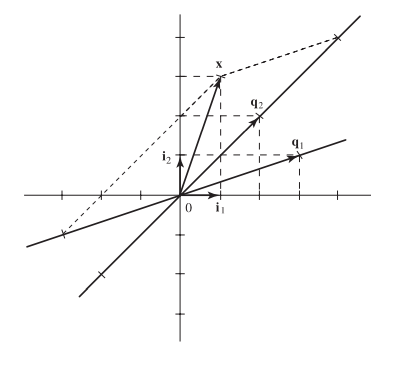
\includegraphics[width = .8\textwidth]{a3.1.PNG}}
\centerline
\par
From the above figure, The three vectors $\boldsymbol{q}_{1}=\left[\begin{array}{ll}3 & 1\end{array}\right]^{\prime}, \boldsymbol{i}_{2}=\left[\begin{array}{ll}0 & 1\end{array}\right]^{\prime}$ and $\boldsymbol{q}_{2}=\left[\begin{array}{ll}2 & 2\end{array}\right]^{\prime}$\\
The representation of $x$ with respect to $\left\{\boldsymbol{q}_{1}, \boldsymbol{i}_{2}\right\}$ is $\left[\begin{array}{ll}\frac{1}{3} & \frac{8}{3}\end{array}\right]^{\prime}$\\
The representation of $\boldsymbol{q}_{1}$ with respect to $\left\{\boldsymbol{i}_{2}, \boldsymbol{q}_{2}\right\}$ is $\left[\begin{array}{ll}-2 & \frac{3}{2}\end{array}\right]^{\prime}$\\
These can be verified like this:
$$
x=\left[\begin{array}{l}
1 \\
3
\end{array}\right]=\left[\begin{array}{ll}
\boldsymbol{q}_{1} & \boldsymbol{i}_{2}
\end{array}\right]\left[\begin{array}{l}
\frac{1}{3} \\
\frac{8}{3}
\end{array}\right]=\left[\begin{array}{ll}
3 & 0 \\
1 & 1
\end{array}\right]\left[\begin{array}{l}
\frac{1}{3} \\
\frac{8}{3}
\end{array}\right]
$$
\section*{3.2}
\subsection*{\rmnum{1}:The norm of $x_{1}$}
1-norm: $\left\|x_{1}\right\|_{1}=\sum_{i=1}^{3}\left|x_{i}\right|=|2|+|-3|+|1|=6$\\
2 -norm: $\left\|\boldsymbol{x}_{1}\right\|_{2}=\left(\sum_{i=1}^{3}\left|x_{i}\right|^{2}\right)^{\frac{1}{2}}=\sqrt{2^{2}+|-3|^{2}+1^{2}}=\sqrt{14}$\\
infinite-norm: $\left\|\boldsymbol{x}_{1}\right\|_{\infty}=\max _{i}\left|x_{i}\right|=3$\\\
\subsection*{\rmnum{2}:The norm of $x_{2}$}
1 -norm: $\left\|\boldsymbol{x}_{2}\right\|_{1}=\sum_{i=1}^{3}\left|x_{i}\right|=|1|+|1|+|1|=3$\\
2-norm: $\left\|\boldsymbol{x}_{2}\right\|_{2}=\left(\sum_{i=1}^{3}\left|x_{i}\right|^{2}\right)^{\frac{1}{2}}=\sqrt{1^{2}+1^{2}+1^{2}}=\sqrt{3}$\\
infinite-norm: $\left\|\boldsymbol{x}_{2}\right\|_{\infty}=\max _{i}\left|x_{i}\right|=1$\\

\section*{3.3}
This is just the orthonormalization procedure.
$$
\left\{\begin{array}{ll}
u_{1}=\alpha_{1} & q_{1}=u_{1} /\left\|u_{1}\right\| \\
u_{2}=\alpha_{2}-\left(q_{1}^{\prime} \alpha_{2}\right) q_{1} & q_{2}=u_{2} /\left\|u_{2}\right\|
\end{array}\right.
$$
This is the ordinary method,what we find is the two vector are orthogonal. so,we just need to make the length of vector is 1 .
$$
\begin{array}{c}
q_{1}=\frac{u_{1}}{\left\|u_{1}\right\|}=\left[\frac{2}{\sqrt{14}}-\frac{3}{\sqrt{14}} \quad \frac{1}{\sqrt{14}}\right]^{\prime} \\
q_{1}=\frac{u_{2}}{\left\|u_{2}\right\|}=\left[\frac{1}{\sqrt{3}} \quad \frac{1}{\sqrt{3}} \quad \frac{1}{\sqrt{3}}\right]^{\prime}
\end{array}
$$

\section*{3.4}
\subsection*{a}
if n>m,$\boldsymbol{AA}^{'}$ is a ordinary vector,which has the rank m\\
\subsection*{b}
if m=n,so $\boldsymbol{A}$ is a nonsingular square matrix,we already have $\boldsymbol{A}^{'}\boldsymbol{A}=\boldsymbol{I}_m$,so $\boldsymbol{A}'=\boldsymbol{A}^{-1}$.
$\boldsymbol{AA}^{'}=\boldsymbol{A}\boldsymbol{A}^{-1}=\boldsymbol{I}_n$

\section*{3.5}
Accoridng to the principle:\\
\[Nillity(\boldsymbol{A})=number of columns of \boldsymbol{A}-rank\boldsymbol(A)\]
\subsection*{\rmnum{1}:}
Rank $\boldsymbol(A_1)=2$\\
Nullity $\boldsymbol(A_1)=3-2=1$
\subsection*{\rmnum{2}:}
Rank $\boldsymbol(A_2)=3$\\
Nullity $\boldsymbol(A_2)=3-3=0$\\
\subsection*{\rmnum{3}:}
Rank $\boldsymbol(A_3)=3$\\
Nullity $\boldsymbol(A_3)=4-3$

\section*{3.6}
For $A_1$:
\begin{equation*}
\boldsymbol{a_1}=
\left[
\begin{array}{c}
1\\
0\\
0
\end{array}
\right]
\boldsymbol{a_2}=
\left[
\begin{array}{c}
0\\
0\\
1\\
\end{array}
\right]
\end{equation*}
The set of $\{\boldsymbol{a_1},\boldsymbol{a_2}\}$ can be the basis of the range spaces.\\
The independent vectors of null space can get by solving the equation:\\
\[\boldsymbol{A}_1 \boldsymbol{\eta}_i=0\]
\begin{equation*}
\boldsymbol{\eta}_1=
\left[
\begin{array}{c}
1\\
0\\
0\\
\end{array}
\right]
\end{equation*}
The set of ${\boldsymbol{\eta}_1}$ is the basis of the null space\\
in the same way,we can get the basis of the range space and null space of $\boldsymbol{A}_2$
\begin{equation*}
\boldsymbol{a_1}=
\left[
\begin{array}{c}
4\\
3\\
1
\end{array}
\right]
\boldsymbol{a_2}=
\left[
\begin{array}{c}
1\\
2\\
1\\
\end{array}
\right]
\boldsymbol{a_3}=
\left[
\begin{array}{c}
-1\\
0\\
0\\
\end{array}
\right]
\end{equation*}
The set of  $\{\boldsymbol{a_1},\boldsymbol{a_2},\boldsymbol{a_3}\}$ is the basis of the range space.\\
because the $\boldsymbol{A}_2$ is full rank,so the basis of the null space is $\{\boldsymbol{0}\}$

\section*{3.7}
\[\rho(\boldsymbol{A})=\rho([\boldsymbol{A}\quad y])=2\]
so a solution $\boldsymbol{x}$ exist with respect to this equation.\\
Because coefficient matrix is full column rank,so the solution is unique.\\
if y=$[1\quad 1\quad 1]^{'}$,$\rho(\boldsymbol{A})=2 \neq \rho([\boldsymbol{A}\quad y])=3$
so,when $\boldsymbol{y}$=$[1 \quad 1\quad 1]^{'}$,the solution is not exist.

\section*{3.8}
$\boldsymbol{x}_p=[0\quad -2\quad 1\quad 1]^{'}$ is a solution, a basis of the null space of $A$:
\[\boldsymbol{A} \boldsymbol{\eta}_i=0\]
\begin{equation*}
\boldsymbol{\eta}_1=
\left[
\begin{array}{c}
1\\
-2\\
1\\
0\\
\end{array}
\right]
\end{equation*}
Thus the gengeral solution can be expressed as:
\[\boldsymbol{x}=\boldsymbol{x}_p+\alpha_1 \boldsymbol{\eta}_1\]

\section*{3.9}
From the example 3.3,we can know the gengeral solution is:
\begin{equation*}
\boldsymbol{x}=
\left[
\begin{array}{c}
\alpha_1\\
-4+\alpha_1+2\alpha_2\\
-\alpha_1\\
-\alpha_2
\end{array}
\right]
\end{equation*}
\[\left\|\boldsymbol{x}\right\|_2=\sqrt{\alpha_1^2+(\alpha_1+2*\alpha_2-4)^2+\alpha_1^2+\alpha_2^2}\]
adjusting polynomials into sum of squares:
\[\sqrt{3(\alpha_1+\frac{2}{3}(\alpha_2-2))^2+\frac{11}{3}(\alpha_2-\frac{16}{11})^2+\frac{32}{11}-(\frac{16}{11})^2}\]
When all the square terms are zero, the Euclidean norm of the solution is the smallest
so,we can get
\[
\left\{
\begin{aligned}
&\alpha_1=\frac{4}{11}& \\   
&\alpha_2=\frac{16}{11}&
\end{aligned}
\right.
\]
so the solution,which can get the smallest Euclidean is :
\begin{equation*}
\boldsymbol{x}=
\left[
\begin{array}{c}
\frac{4}{11}\\
-\frac{8}{11}\\
-\frac{4}{11}\\
-\frac{16}{11}
\end{array}
\right]
\end{equation*}


\end{document}